\section{DRAM Class Reference}
\label{classDRAM}\index{DRAM@{DRAM}}
{\tt \#include $<$dram.h$>$}

Inheritance diagram for DRAM:\nopagebreak
\begin{figure}[H]
\begin{center}
\leavevmode
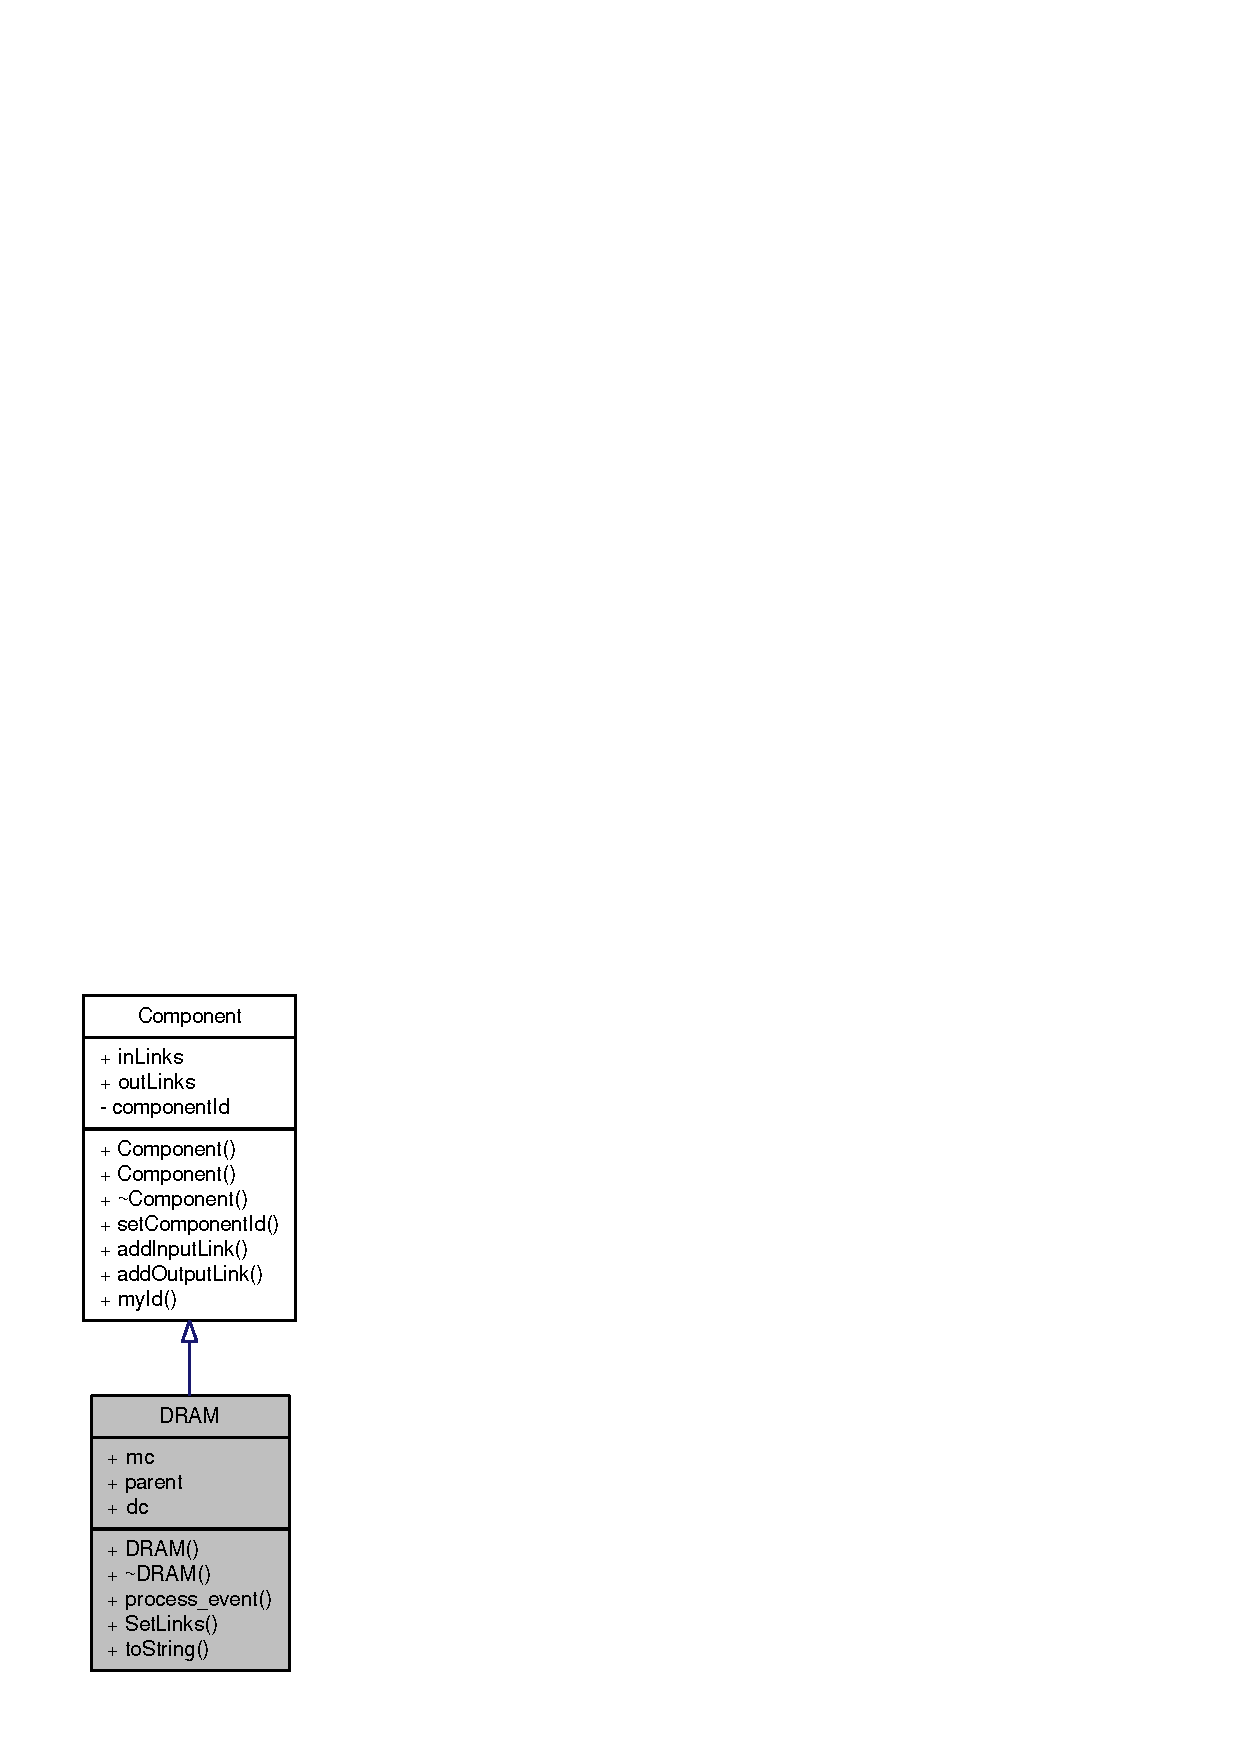
\includegraphics[width=146pt]{classDRAM__inherit__graph}
\end{center}
\end{figure}
Collaboration diagram for DRAM:\nopagebreak
\begin{figure}[H]
\begin{center}
\leavevmode
\includegraphics[height=400pt]{classDRAM__coll__graph}
\end{center}
\end{figure}
\subsection*{Public Member Functions}
\begin{CompactItemize}
\item 
{\bf DRAM} ()
\item 
{\bf $\sim$DRAM} ()
\item 
void {\bf process\_\-event} ({\bf IrisEvent} $\ast$e)
\item 
void {\bf SetLinks} ()
\item 
std::string {\bf toString} ()
\end{CompactItemize}
\subsection*{Public Attributes}
\begin{CompactItemize}
\item 
{\bf Component} $\ast$ {\bf mc}
\item 
{\bf Component} $\ast$ {\bf parent}
\item 
{\bf DRAMChannel} {\bf dc} [{\bf NO\_\-OF\_\-CHANNELS}]
\end{CompactItemize}


\subsection{Detailed Description}


Definition at line 70 of file dram.h.

\subsection{Constructor \& Destructor Documentation}
\index{DRAM@{DRAM}!DRAM@{DRAM}}
\index{DRAM@{DRAM}!DRAM@{DRAM}}
\subsubsection[{DRAM}]{\setlength{\rightskip}{0pt plus 5cm}DRAM::DRAM ()}\label{classDRAM_d2edaff90ae758b53179bfa09075af9b}




Definition at line 36 of file dram.cc.

References dc, DRAMChannel::dramBankBusyCycles, DRAMChannel::dramBankBusyTime, DRAMChannel::dramBusyCycles, DRAMChannel::dramBusyTime, NO\_\-OF\_\-BANKS, NO\_\-OF\_\-CHANNELS, and NO\_\-OF\_\-RANKS.\index{DRAM@{DRAM}!$\sim$DRAM@{$\sim$DRAM}}
\index{$\sim$DRAM@{$\sim$DRAM}!DRAM@{DRAM}}
\subsubsection[{$\sim$DRAM}]{\setlength{\rightskip}{0pt plus 5cm}DRAM::$\sim$DRAM ()}\label{classDRAM_0d19f4410081d5e4b807d64ba688511f}




Definition at line 68 of file dram.cc.

\subsection{Member Function Documentation}
\index{DRAM@{DRAM}!process\_\-event@{process\_\-event}}
\index{process\_\-event@{process\_\-event}!DRAM@{DRAM}}
\subsubsection[{process\_\-event}]{\setlength{\rightskip}{0pt plus 5cm}void DRAM::process\_\-event ({\bf IrisEvent} $\ast$ {\em e})}\label{classDRAM_a7fa043a15cf99d7916e0edb98546af5}




Definition at line 90 of file dram.cc.\index{DRAM@{DRAM}!SetLinks@{SetLinks}}
\index{SetLinks@{SetLinks}!DRAM@{DRAM}}
\subsubsection[{SetLinks}]{\setlength{\rightskip}{0pt plus 5cm}void DRAM::SetLinks ()}\label{classDRAM_81ed024032a90e5cb7583aeffa1b2d72}




Definition at line 73 of file dram.cc.

References DRAMChannel::child, dc, mc, DRAMChannel::mc, NO\_\-OF\_\-CHANNELS, parent, and DRAMChannel::parent.

Referenced by MC::Init().

Here is the caller graph for this function:\nopagebreak
\begin{figure}[H]
\begin{center}
\leavevmode
\includegraphics[width=148pt]{classDRAM_81ed024032a90e5cb7583aeffa1b2d72_icgraph}
\end{center}
\end{figure}
\index{DRAM@{DRAM}!toString@{toString}}
\index{toString@{toString}!DRAM@{DRAM}}
\subsubsection[{toString}]{\setlength{\rightskip}{0pt plus 5cm}std::string DRAM::toString ()}\label{classDRAM_838b2e78677227b519959a20f12557f0}




\subsection{Member Data Documentation}
\index{DRAM@{DRAM}!dc@{dc}}
\index{dc@{dc}!DRAM@{DRAM}}
\subsubsection[{dc}]{\setlength{\rightskip}{0pt plus 5cm}{\bf DRAMChannel} {\bf DRAM::dc}[{\bf NO\_\-OF\_\-CHANNELS}]}\label{classDRAM_7c519dc9331a72179a64d22c6cc206d1}




Definition at line 77 of file dram.h.

Referenced by DRAM(), and SetLinks().\index{DRAM@{DRAM}!mc@{mc}}
\index{mc@{mc}!DRAM@{DRAM}}
\subsubsection[{mc}]{\setlength{\rightskip}{0pt plus 5cm}{\bf Component}$\ast$ {\bf DRAM::mc}}\label{classDRAM_6544971f785eab4c76b48f675debe55e}




Definition at line 75 of file dram.h.

Referenced by MC::Init(), and SetLinks().\index{DRAM@{DRAM}!parent@{parent}}
\index{parent@{parent}!DRAM@{DRAM}}
\subsubsection[{parent}]{\setlength{\rightskip}{0pt plus 5cm}{\bf Component}$\ast$ {\bf DRAM::parent}}\label{classDRAM_f4aae723a8f9516ce1fefb4427bdee4f}




Definition at line 76 of file dram.h.

Referenced by MC::Init(), and SetLinks().

The documentation for this class was generated from the following files:\begin{CompactItemize}
\item 
{\bf dram.h}\item 
{\bf dram.cc}\end{CompactItemize}
